\section{Errori nel calcolo di funzioni non razionali}
Nel caso in cui si abbia a che fare con \textbf{funzioni non razionali} dobbiamo, prima di procedere al
calcolo in macchina, approssimarla con una funzione razionale.

Dobbiamo quindi trovare una funzione $h$ che approssima $f$, la quale introduce un nuovo tipo di errore, detto
\textbf{errore analitico} dato dalla formula
\[ \ean = \frac{h(x) - f(x)}{f(x)} \]
Un possibile modo di approssimare la funzione $f$ è tramite lo sviluppo di Taylor arrestato ad un certo ordine.

In questo corso non trattiamo l'errore analitico ma siamo comunque interessati all'analisi dell'errore inerente
e algoritmico di funzioni non razionali.

\begin{example}
	Studiamo il condizionamento della funzione
	\[ f(x) = \frac{e^x - 1}{x} \]
	per $x \to 0^+$. Come sappiamo l'errore inerente, in un'analisi al primo ordine, equivale a
	\[ \ein = \frac{f'(x)}{f(x)} \epsilon_x x \]
	Mentre l'errore di rappresentazione sul dato iniziale equivale a
	\[ \epsilon_x = \frac{\tx - x}{x} \]
	con $|\epsilon_x| \leq u$. Per prima cosa dobbiamo calcolare la derivata della funzione $f$
	\[ f'(x) = \frac{x e^x - 1 (e^x - 1)}{x^2} = \frac{x e^x - e^x + 1}{x^2} \]
	Possiamo ora calcolare il coefficienti di amplificazione
	\[
		c_x = \frac{f'(x)}{f(x)} x =
		\frac{x e^x - e^x + 1}{x^2} \frac{x}{e^x - 1} x =
		\frac{x e^x - e^x + 1}{e^x - 1}
	\]
	Il limite per $x \to 0^+$, come possiamo notare, è un caso di indeterminazione
	\[ \lim_{x \to 0^+} \frac{x e^x - e^x + 1}{e^x - 1} = \frac{0}{0} \]
	risolvibile con il teorema di de l'H\^ospital calcolando il limite
	\[ \lim_{x \to 0^+} \frac{e^x + x e^x - e^x}{e^x} = \lim_{x \to 0^+} x = 0 \]
	Concludiamo quindi che il problema per $x \to 0^+$ è perfettamente ben condizionato.
\end{example}

\begin{example}
	Calcoliamo l'errore algoritmico della funzione
	\[ f(x) = \frac{e^x - 1}{x} \]
	assumendo di avere a disposizione una funzione di macchina \verb|Exp| tale che
	\[ \text{Exp} (x) = e^x (1 + \epsilon) \]
	con $|\epsilon| \leq u$. La funzione effettivamente calcolata in macchina è quindi
	\[
		g(x) = (\text{Exp} (x) \ominus 1) \oslash x =
		\frac{(e^x (1 + \epsilon_1) - 1) (1 + \epsilon_2)}{x} (1 + \epsilon_3)
	\]
	Da qui possiamo procedere con un'analisi in avanti dell'errore
	\begin{center}
		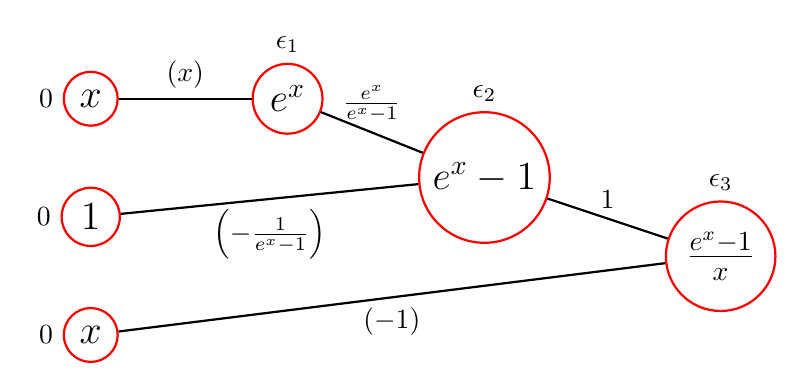
\begin{tikzpicture}[mynode/.style={draw=red, thick, circle, font=\Large}]
			\node[mynode, label=left:$0$] at (0, 1.5) (x1) {$x$};
			\node[mynode, label=left:$0$] at (0, 0) (1) {$1$};
			\node[mynode, label=left:$0$] at (0, -1.5) (x2) {$x$};

			\node[mynode, label=above:$\epsilon_1$] at (2.5, 1.5) (e^x) {$e^x$};
			\node[mynode, label=above:$\epsilon_2$] at (5, 0.5) (e^x-1) {$e^x - 1$};
			\node[mynode, label=above:$\epsilon_3$] at (8, -0.5) (e^x-1/x) {$\frac{e^x-1}{x}$};

			\path
			(x1) edge[thick] node[above, black] {$(x)$} (e^x)
			(e^x) edge[thick] node[above, black] {$\frac{e^x}{e^x-1}$} (e^x-1)
			(1) edge[thick] node[below, black] {$\left( -\frac{1}{e^x-1} \right)$} (e^x-1)
			(e^x-1) edge[thick] node[above, black] {$1$} (e^x-1/x)
			(x2) edge[thick] node[below, black] {$(-1)$} (e^x-1/x);
		\end{tikzpicture}
	\end{center}
	Dalla quale otteniamo
	\begin{align*}
		\ealg =   & \epsilon_3 + 1 \left( \epsilon_2 + \frac{e^x}{e^x - 1} \epsilon_1 \right)              \\
		|\ealg| = & \left| \epsilon_3 + 1 \left( \epsilon_2 + \frac{e^x}{e^x-1} \epsilon_1 \right) \right| \\
		\leq      & |\epsilon_3| + |\epsilon_2| + \left| \frac{e^x}{e^x-1} \right| \left|\epsilon_1\right| \\
		\leq      & 2u + \frac{e^x}{|e^x - 1|} u
	\end{align*}
	Concludiamo quindi che l'algoritmo è numericamente instabile quando $x$ tende a 0 da destra poiché
	\[ \lim_{x \to 0^+} \frac{e^x}{|e^x-1|} = +\infty \]
\end{example}
